
%%%%%%%%%%%%%%%%%%%%%%% file typeinst.tex %%%%%%%%%%%%%%%%%%%%%%%%%
%
% This is the LaTeX source for the instructions to authors using
% the LaTeX document class 'llncs.cls' for contributions to
% the Lecture Notes in Computer Sciences series.
% http://www.springer.com/lncs       Springer Heidelberg 2006/05/04
%
% It may be used as a template for your own input - copy it
% to a new file with a new name and use it as the basis
% for your article.
%
% NB: the document class 'llncs' has its own and detailed documentation, see
% ftp://ftp.springer.de/data/pubftp/pub/tex/latex/llncs/latex2e/llncsdoc.pdf
%
%%%%%%%%%%%%%%%%%%%%%%%%%%%%%%%%%%%%%%%%%%%%%%%%%%%%%%%%%%%%%%%%%%%


\documentclass[runningheads,a4paper]{llncs}
\usepackage[a4paper, total={6in, 8in}]{geometry}
\usepackage{amssymb}
\setcounter{tocdepth}{3}
\usepackage{graphicx}
\usepackage{subcaption}
\usepackage{listings}
%\lstset{
%	numbers=left
%	language=Java
%	frame=single,
%	breaklines=true,
	%postbreak=\raisebox{0ex}[0ex][0ex]{\ensuremath{\color{red}\hookrightarrow\space}}
%}
\renewcommand{\lstlistingname}{Code}

\captionsetup{compatibility=false}

\usepackage{url}
\urldef{\mailsa}\path|{alfred.hofmann, ursula.barth, ingrid.haas, frank.holzwarth,|
\urldef{\mailsb}\path|anna.kramer, leonie.kunz, christine.reiss, nicole.sator,|
\urldef{\mailsc}\path|erika.siebert-cole, peter.strasser, lncs}@springer.com|    
\newcommand{\keywords}[1]{\par\addvspace\baselineskip
\noindent\keywordname\enspace\ignorespaces#1}

\begin{document}

\mainmatter  


\newpage
\tableofcontents
\newpage

\abstract{
The implementation of parallel computing on the integral of a function by Monte
Carlo method is described in this assignment. Particularly, the assignment exploits the Fast-
Flow parallel framework and C++ threads for building stream parallelism including pipeline
and farm. The experiments illustrate the comparison of time consuming of these ways with
different interval numbers, a set of functions and a various threads.
} 

\section{Introduction}
\label{sec:intro}
% Describe that dataset and generally about sections


With the development of hardware technologies and a plenty of data, the requirement of time
consuming to process or compute some tasks have been noticed, which leads to the growth
of parallelism. The parallelism tasks are divided into some parts such as: stream parallelism,
data parallelism, task parallelism and so on.
This assignment is about exploiting the stream parallelism on computing integral of a given
function with Monte Carlo method. Because of a stream of interval numbers from the re-
quirement of the project, a stream parallelism with pipeline and farm is utilized to parallel
computing the Monte Carlo method for each interval number. To construct a stream par-
allelism structure, the FastFlow (FF) framework and C++ threads are mentioned in this
assignment.


The remaining of the assignment is constructed: the Section~\ref{sec:imple} describes about the imple-
mentation of computing the integral of a given function with Monte Carlo. The results and
experiments using FF and C++ threads are represented in Section~\ref{sec:exper}, while Section~\ref{Conc} concludes
the assignment.


%The remaining of the assignment is constructed: the Section~\ref{sec:imple} describes about the implementation of computing the integral of a given function with Monte Carlo. 
%The results and experiments using FF and C++ threads are represented in Section~\ref{sec:exper}, while Section~\ref{Conc} concludes the assignment.
	
\section{Implementation}
\label{sec:imple}

In this part of the report, the general idea of the Monte Carlo in computation of a integral
function is designed by FF framework and C++ threads. The basic idea is about forming an
interval number object with basic fields (a range of the interval number, a random number
(N), list of N random numbers, Monte Carlo number of this interval and an ID for sorting)
and methods. Hence, each interval number goes through each stage which executes specific
tasks in stream parallelism built by FF and C++ threads.


\subsection{FastFlow}
\label{subsec:ff}

\begin{figure*}[h!]
	\centering
	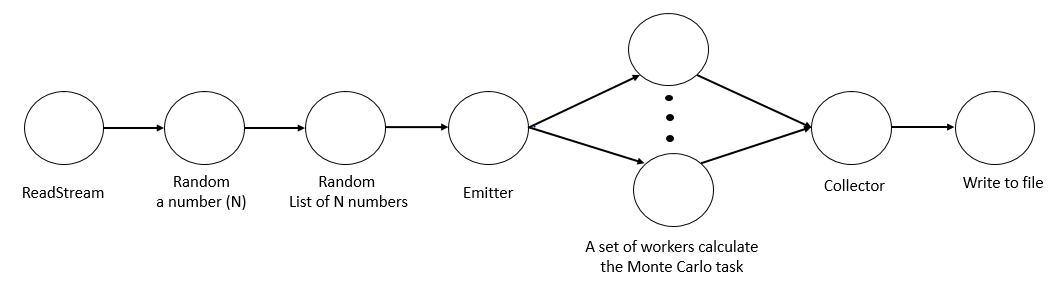
\includegraphics[scale = 0.4]{image/ffStructure}	
	\caption{The diagram of FF structure}
	\label{Fig:ffStructure}
\end{figure*}

To build a parallelism, the FF a structured parallel programming framework~\cite{fastflow} is utilized
because of plenty of advantages such as highly efficient stream parallel and a set of ready-to-
use for programmers. In addition, FF can be flexible for creation complex parallelism with a
lot of different nodes.
With the Monte Carlo task, the FF framework is used to build a stream parallelism with
pipeline and farm. Particularly, from the Fig~\ref{Fig:ffStructure}, it can be clear that the structure is built based
on a set of stages including: reading a set of interval numbers, choosing a random number (N),
choosing a list of N random numbers, setting Monte Carlo number calculations to threads and
writing to a file.
Generally, each stage has a specific task to resolve. Because of the convenience of FF, each of
stage or task or node is implemented as a function. However, if the a stage has more than one
input or output, it can be redefined. In more detail, the tasks of stages is described:

\begin{itemize}
\item readStream: takes a couple numbers at each time from a stream of file.
\item random a number (N): randomly selects a number.
\item random a list of N numbers: is generated from this stages.
\item emitter: split interval numbers to free workers.
\item a set of workers: compute Monte Carlo method for set of interval numbers.
\item collector: takes bunch of interval numbers and send to the next stage.
\item write to file: write the Monte Carlo to a file.
\end{itemize}

\subsection{C++ Thread}
\label{subsec:thread}

\begin{figure*}[h!]
	\centering
	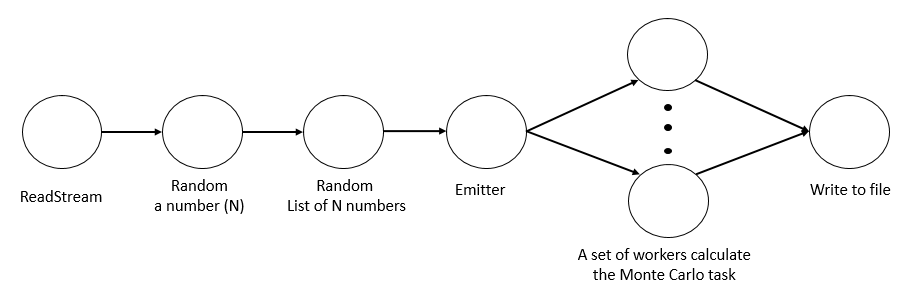
\includegraphics[scale = 0.4]{image/threadStructure}	
	\caption{The diagram of C++ threads structure}
	\label{Fig:threadStructure}
\end{figure*}

In case of using C++ threads, a similar construction is built with pipeline and farm on stream
parallelism (in the Fig~\ref{Fig:threadStructure}). 
However, without supporting from FF, the communication between
stages is executed through queues and combination of mutex and condition variable in C++~\cite{thread}.
In more detail, the queues run a role like containers which hold interval numbers executed
from previous stage and waiting the next call of the next stage. Meanwhile, the mutex and
condition variable are similar to doors and bells, respectively. Particularly, to start a stage
from a thread, the mutex is used to lock the thread. After a stage has completed its task, the
thread is unlocked by the mutex and sends a notify to next threads waiting for their turns.
Based on some conditions, the notified threads can be waken up for their tasks or still sleep.
In addition, each stage in case of C++ threads is implemented by a thread with a specific task
like FF construction. The general idea of stream parallelism in C++ threads construction is
quite similar the way of FF construction. Nevertheless, at the last stage, the C++ threads
construction uses a queue to contain results of workers, in stead of using a collector to gather
output of workers from farm. Then the final stage pops each result from queue to a file. Before
writing the result to the file, the Monte Carlo numbers are sorted based on the ID of interval
numbers.



%Each of the output of stage or thread is a queue from which the next stage can take sequential objects to compute.
%However, it exists some problems in case of race condition.
%Therefore, the mutex ... and condition variable techniques are utilized to lock and unlock some data.
%In case of using C++ threads implementing this task, 
%For a parallelism 
%http://www.cplusplus.com/reference/thread/thread/
%threads ....
%condition variable 
%mutex...


\section{Experiments}
\label{sec:exper}
The experiments of the Monte Carlo task with FF framework and C++ threads are mentioned
in this section. Particularly, a set of different functions in Table 1 (with powers from 5 to 10) tried, while streams of interval numbers are generated randomly including 100 and 2000
interval numbers with a in [1, 1000] and b in [a, 1500]. Additionally, the assignment considers
many different threads from 6 to 130 in experiments. About the complexity
of construction between FF framework and C++ threads, with the FF, programmers need to
define tasks for every stage of construction and correctly select classes or structures to build the
application, whereas in case of using C++ threads, the programmers is required to clearly
understand the idea of communication between threads.

\begin{table}[]
	\centering
	\caption{List of functions}
	\label{listFunc}
	\begin{tabular}{c|l}
		\hline
		\hline
		Power & Set of Function                                                                                                                                                                                                                  \\ \hline
		
		5     & $x^{5}$ + 2$x^{4}$ + 3$x^{3}$ + 4$x^{2}$ + 5x + 6                                                                                                                            \\ 
		6     & $x^{6}$ + 2$x^{5}$ + 3$x^{4}$ + 4$x^{3}$ + 5$x^{2}$ + 6x + 7                                                                                                    \\ 
		7     & $x^{7}$ + 2$x^{6}$ + 3$x^{5}$ + 4$x^{4}$ + 5$x^{3}$ + 6$x^{2}$ + 7x + 8                                                                            \\ 
		8     & $x^{8}$ + 2$x^{7}$ + 3x$x^{6}$ + 4$x^{5}$ + 5$x^{4}$ + 6$x^{3}$ + 7$x^{2}$ + 8x + 9                                                    \\ 
		9     & $x^{9}$ + 2$x^{8}$ + 3$x^{7}$ + 4$x^{6}$ + 5$x^{5}$ + 6$x^{4}$ + 7$x^{3}$ + 8x\textasciicircum{}2 + 9x + 10                           \\ 
		10    & $x^{10}$ + 2$x^{9}$ + 3$x^{8}$ + 4$x^{7}$ + 5$x^{6}$ + 6$x^{5}$ + 7$x^{4}$ + 8$x^{3}$ + 9$x^{2}$ + 10x + 11 \\ \hline \hline
	\end{tabular}
\end{table}
%The results of experiments are illustrated in Figs 3, 4, 5. In these figures, the vertical axis
%shows the execution time, while the other one is about the power of functions. The solid line
%represents the FF performance, while the dashed line illustrates the performance of C++
%threads.
%It can be clear that in the set of functions, with 100 interval numbers, the C++ threads is
%better than FF framework in case of execution time with the number of threads being 6, 8, 10
%and 15, whereas with the other numbers of threads (20 and 25), the execution time of C++
%threads is similar and higher than FF, respectively.
%Meanwhile, in case of 500 and 1000 interval numbers sets, with a few threads (being 6 threads),
%the performance of C++ threads and FF framework is quite similar to each other. However,
%with larger numbers of threads (8, 10, 15, 20 and 25), the performance of C++ threads
%dominates the performance of FF framework.

\begin{figure*}[t!]
	\centering
	\begin{subfigure}[b]{0.3\textwidth}
		%\centering
		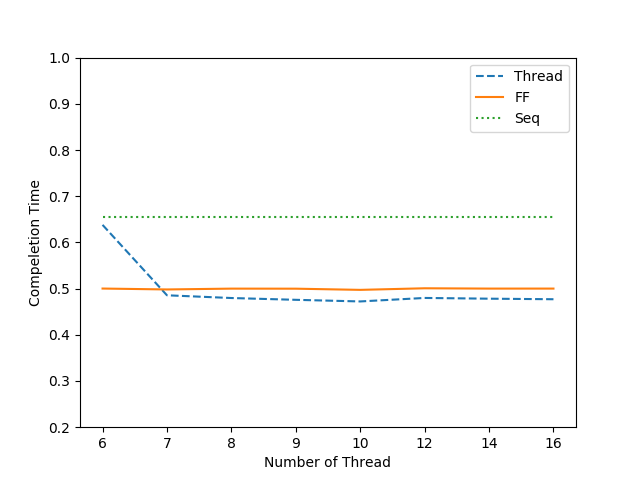
\includegraphics[scale = 0.3]{image/graph/input100/pow05}
		\caption{Power function: 5}
	\end{subfigure}
	\begin{subfigure}[b]{0.3\textwidth}
		%\centering
		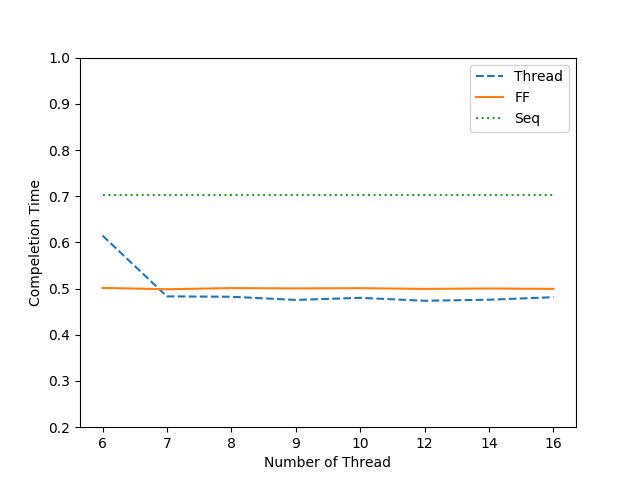
\includegraphics[scale = 0.3]{image/graph/input100/pow06}
		\caption{Power function: 6}
	\end{subfigure}
	\begin{subfigure}[b]{0.3\textwidth}
		%\centering
		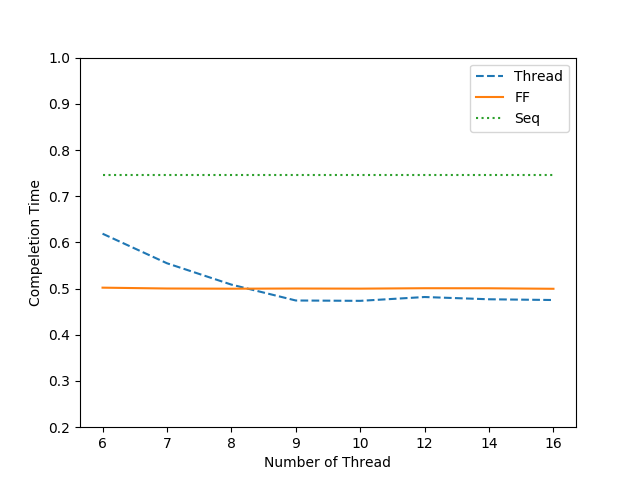
\includegraphics[scale = 0.3]{image/graph/input100/pow07}
		\caption{Power function: 7}
	\end{subfigure}
	\begin{subfigure}[b]{0.3\textwidth}
		%\centering
		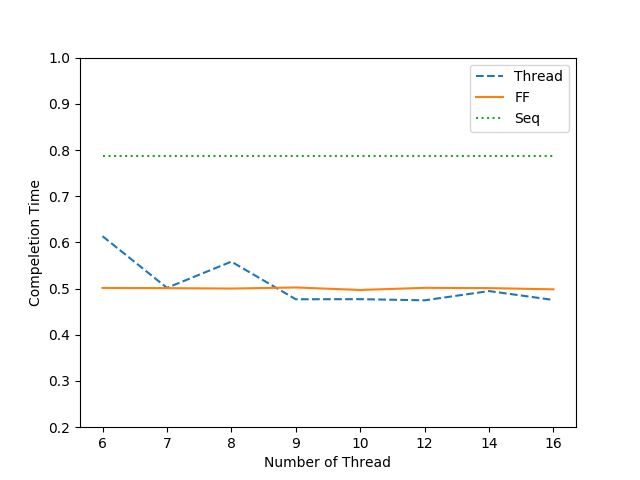
\includegraphics[scale = 0.3]{image/graph/input100/pow08}
		\caption{Power function: 8}
	\end{subfigure}
	\begin{subfigure}[b]{0.3\textwidth}
		%\centering
		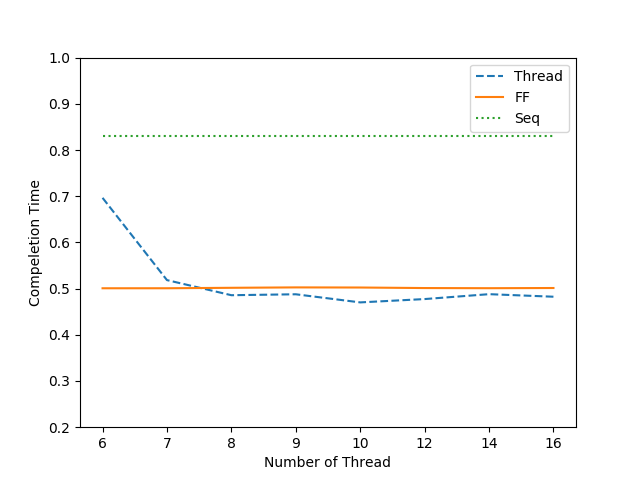
\includegraphics[scale = 0.3]{image/graph/input100/pow09}
		\caption{Power function: 9}
	\end{subfigure}
	\begin{subfigure}[b]{0.3\textwidth}
		%\centering
		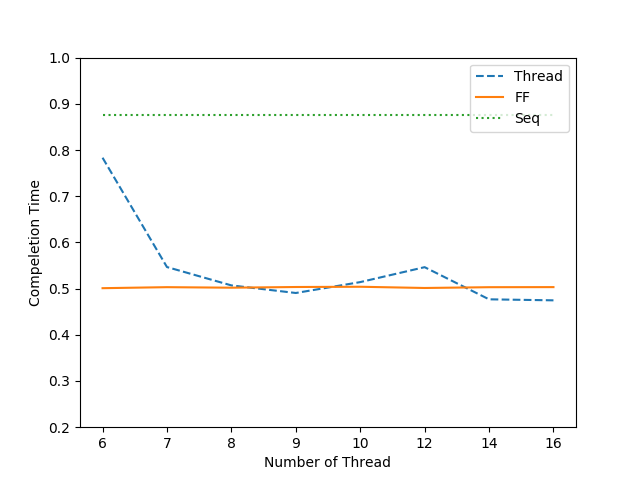
\includegraphics[scale = 0.3]{image/graph/input100/pow10}
		\caption{Power function: 10}
	\end{subfigure}
	\caption{Graph of completion time in different functions with 100 interval numbers}
	\label{Fig:powFunc}
\end{figure*}
The first experiment on Fig~\ref{Fig:powFunc} illustrates the difference of functions on the Table~\ref{listFunc}. The vertical and horizontal axes are the completion time and the number of threads, respectively.
From this experiment, it can be seen that there are not too much different from these functions. Therefore, the next experiment choose a fixed function. In this case, the function  ``$x^{7}$ + 2$x^{6}$ + 3$x^{5}$ + 4$x^{4}$ + 5$x^{3}$ + 6$x^{2}$ + 7x + 8'' is selected.


%In the Fig~\ref{Fig:b}, the result of farm is lower (better) than the latency of the model from sequentiality because it can be a reason that with a processor, the data which fit to this process's cache is quite small, need some time for read and write to the main memory.
%However, in the general application, the completion time of model is lower (better) in case of more and more number of threads. 
%The reason can be the bottle neck in the pipeline and the time of communication between stages in the application.
In the Fig~\ref{Fig:2000_130}, the experiment is displayed through the vertical and horizontal axes with completion time and the number of threads, respectively.
In particular, with one worker in a farm stage, the completion time of C++ threads quite similar to the completion time of sequentiality because it reduces some time with pipeline and introduces some overhead from communication between stages, creating and termination threads. Then, when the number of workers increases from two to twenty, the completion time of C++ threads drops, but the level of decrease cannot be exactly equal to the predictive version due to the overhead of other stages. Meanwhile, in the farm stage in the Fig~\ref{Fig:b}, the latency of C++ threads is better than the predictive because with a processor, the data which fit to this process's cache is quite small, need some time for read and write to the main memory, whereas in case of more processor (more cache) the time for reading and writing from main memory can be eliminated or reduced.
After falling, the completion time of C++ thread reaches the plateau when the number of workers rises until under forty, before slowly rising and soaring. Due to the increase of latency of farm stage, the completion time of the C++ threads goes up with the number of worker is greater than around 25.

\begin{figure*}[t!]
	\centering
	\begin{subfigure}[b]{0.4\textwidth}
		%\centering
		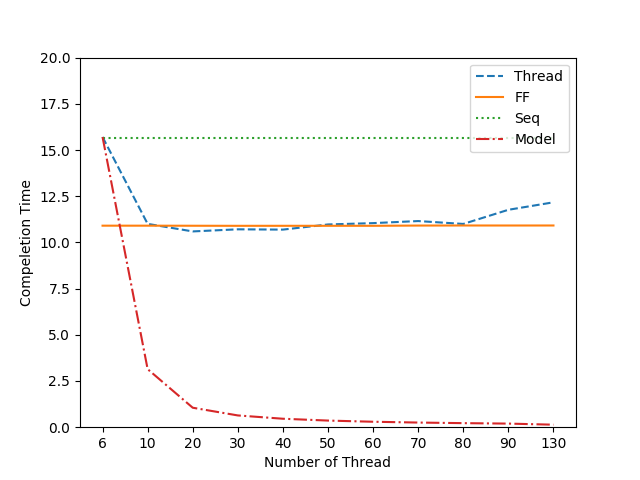
\includegraphics[scale = 0.4]{image/graph/pow07_2000_0_130_perfect}
		\caption{Completion time of application}
		\label{Fig:a}
	\end{subfigure}
	\begin{subfigure}[b]{0.4\textwidth}
		%\centering
		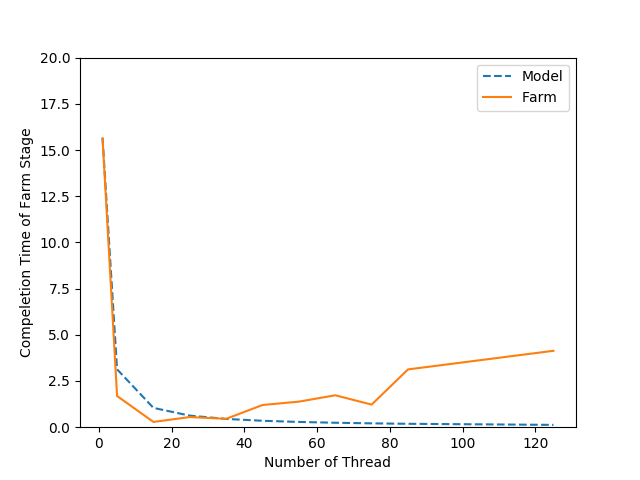
\includegraphics[scale = 0.4]{image/graph/Farm_pow07_2000_0_130_perfect}
		\caption{Completion time of Farm stage}
		\label{Fig:b}
	\end{subfigure}
	\caption{Graph of completion time in case of whole application and farm stage with 2000 interval numbers and power of function being 7}
	\label{Fig:2000_130}
\end{figure*}


\section{Conclusion}
\label{Conc}
The computation of integral of a given function with Monte Carlo method from a stream of
interval numbers is implemented with stream parallelism. In more detail, the implementation
is built based on the combination of pipeline and farm with two different technologies such
as FF framework and C++ threads. The comparison of these techniques can be clear that in
case of time performance, the C++ threads is better than FF framework. Nevertheless, the
construction of FF framework is less complex than using C++ threads.
are

\section{Ackowledgements}
I would like to show my gratitude to Prof. Marco Danelutto and his Assistant Dr. Massimo Torquati about lessons in Distributed systems: paradigms and models course at University of Pisa.
Additionally, I say thank to my friends who support and encourage me in this course.

\bibliography{Ref}
\bibliographystyle{bibfile}


\section{Compiling and Runing}
To compile the source code of these implementations on the server, the Cmake is utilized as below.
\begin{lstlisting}[numbers=left,language=Java,frame=single,breaklines=false,label=SelfishAlgorithm.]
$ mkdir build
$ cd build
$ cmake ..
$ make
\end{lstlisting}
To running these implementations, the same number of parameters are used.
\begin{lstlisting}[numbers=left,language=Java,frame=single,breaklines=false,label=SelfishAlgorithm]
./ff <NoThread><IntervalNumberFile><PowerFunc><ElementFunction>
./threads <NoThread><IntervalNumberFile><PowerFunc><ElementFunction>
./seq <IntervalNumberFile><PowerFunc><ElementFunction>
\end{lstlisting}
For example, the FF framework and C++ threads are executed with 10 threads, a path of
Interval Number File ``../input/Input.txt'', and a given function “$x^{3} + 5x^{2} + 2x +1$.
\begin{lstlisting}[numbers=left,language=Java,frame=single,breaklines=false,label=SelfishAlgorithm]
./ff 10 ../input/Input.txt 3 1 5 2 1
./threads 10 ../input/Input.txt 3 1 5 2 1
./seq ../input/Input.txt 3 1 5 2 1
\end{lstlisting}
\end{document}

\iffals

\section{Metrics and Activation}
\label{Metrics}
\subsection{Sigmoid}
\subsection{Activation Function}
\subsection{Identity Function}
\subsection{UnitStep}
\section{Cross-Validation}
\label{CV}



\begin{figure*}[t!]
	\centering
	\begin{subfigure}[b]{0.6\textwidth}
		%\centering
		
\includegraphics[scale = 0.6]{image/Unipi_Image}
		\caption{In-degree distribution with an exponent 4.5}
	\end{subfigure}
	\\
	\begin{subfigure}[b]{0.6\textwidth}
		%\centering
		
\includegraphics[scale = 0.6]{image/Unipi_Image}
		\caption{Out-degree distribution with an exponent 5.5}
	\end{subfigure}
	\caption{In-degree and Out-degree distributions}
		\label{Fig:Distri}
\end{figure*}
\textbf{Second Part}:
\begin{figure*}[t!]
	\centering
	\begin{subfigure}[b]{0.6\textwidth}
		%\centering
		
\includegraphics[scale = 0.6]{image/Unipi_Image}
		\caption{Size of WCC distribution with an exponent 10 of power law}
	\end{subfigure}
	\\
	\begin{subfigure}[b]{0.6\textwidth}
		%\centering
		
\includegraphics[scale = 0.6]{image/Unipi_Image}
		\caption{Size of SCC distribution with an exponent 9 of power law}
	\end{subfigure}

	\caption{Size of WCC and SCC distributions}
		\label{Fig:WCC_SCC}
\end{figure*}

\begin{figure*}[t!]

	\centering
	\begin{subfigure}[b]{0.6\textwidth}
		%\centering
		
\includegraphics[scale = 0.6]{image/Unipi_Image}
		\caption{Experiment with BFS on forward direction}
	\end{subfigure}
	\\
	\begin{subfigure}[b]{0.6\textwidth}
		%\centering
		
\includegraphics[scale = 0.6]{image/Unipi_Image}
		\caption{Experiment with BFS on backward direction}
	\end{subfigure}
	\\
	\begin{subfigure}[b]{0.6\textwidth}
		%\centering
		
\includegraphics[scale = 0.6]{image/Unipi_Image}
		\caption{Experiment with BFS on both directions}
	\end{subfigure}
	\caption{Experiments of BFS algorithm on three kinds of graph}
		\label{Fig:BFS}
\end{figure*}

\subsection{Mote Carlo Task}
\label{sec:monte}

Monte Carlo methods use randomly numbers to simulate the process and estimate the average result.
In the specific requirement of the project, the integral of a given function is computed based on the Monte Carlo method with a set of different interval numbers.
Therefore, the input includes a stream of intervals (a set of couples of two integer numbers) and a given function.
Then the output or the final Monte Carlo numbers of each interval number is calculated based on the formula followed:
%For computing integral of a given function based on the Monte Carlo,

$$\frac{1}{N}\sum_{i=1}^N(f(x_{i})(b-a))$$

The main idea of parallelism in this task is about parallel computing Monte Carlo for each of interval number.
However, each task is parallel run for different interval number.
For example, in case of reading a new interval number and random a number, after reading a interval number, the next stage (choose a random number) is set a random number for this interval number. Meanwhile, the reading stage takes a new interval number.
Therefore, two threads are running.



\begin{figure*}[t!]
	\centering
	\begin{subfigure}[b]{0.4\textwidth}
		%\centering
		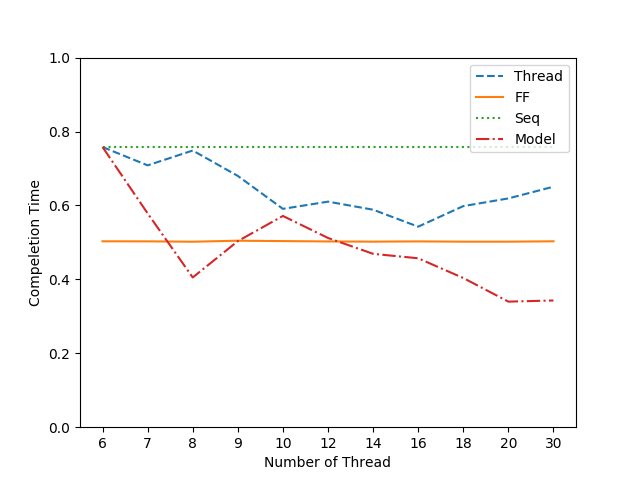
\includegraphics[scale = 0.4]{image/graph/pow07_100_0_30}
		\caption{Completion time of application}
	\end{subfigure}
	\begin{subfigure}[b]{0.4\textwidth}
		%\centering
		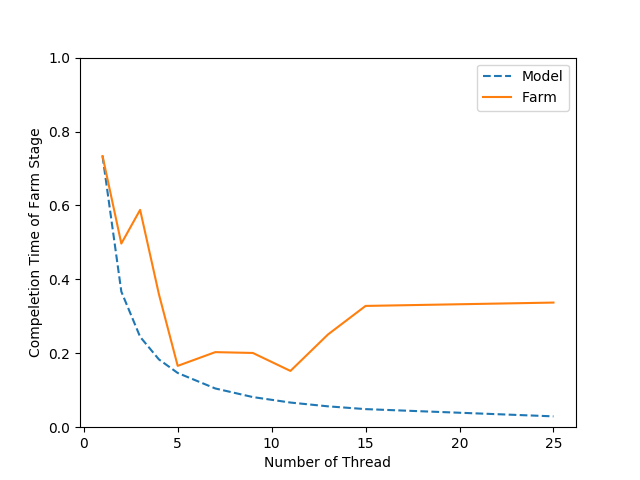
\includegraphics[scale = 0.4]{image/graph/Farm_pow07_100_0_30}
		\caption{Completion time of Farm stage}
	\end{subfigure}
	\caption{Graph of completion time in case of whole application and farm stage with 100 interval numbers and power of function being 7}
	\label{Fig:}
\end{figure*}
\begin{figure*}[t!]
	\centering
	\begin{subfigure}[b]{0.4\textwidth}
		%\centering
		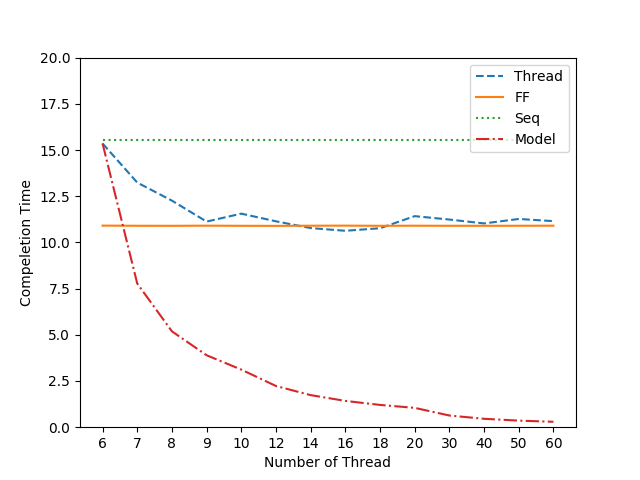
\includegraphics[scale = 0.4]{image/graph/pow07_2000_0_60_perfect}
		\caption{Completion time of application}
	\end{subfigure}
	\begin{subfigure}[b]{0.4\textwidth}
		%\centering
		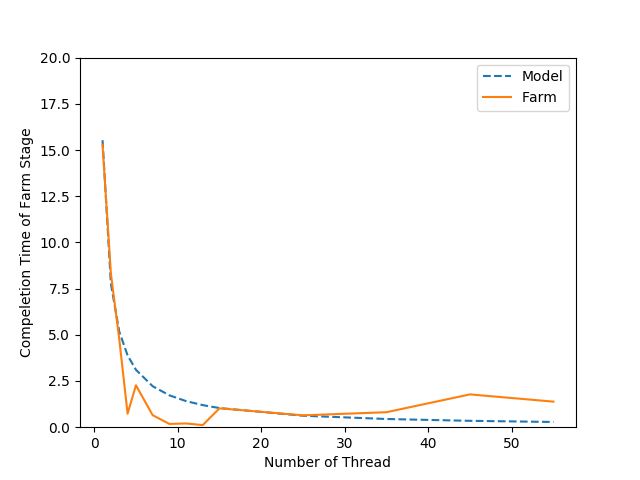
\includegraphics[scale = 0.4]{image/graph/Farm_pow07_2000_0_60_perfect}
		\caption{Completion time of Farm stage}
	\end{subfigure}
	\caption{Graph of completion time in case of whole application and farm stage with 2000 interval numbers and power of function being 7}
	\label{Fig:2000_30}
\end{figure*}
